\documentclass[a4paper,11pt]{article}
\include{../../../latex_headers/lab_header}


% ---------------------------------- Document ----------------------------------
\begin{document}
\pagenumbering{arabic}

\begin{center}
{\Large CMPUT 350 Lab 8 Prep Problems}
\end{center}

% Add important dates, change TA, add TA tools

\linerule


\section*{Geometry Review}
\subsection*{3D Vector Cross-Product}
\centerline{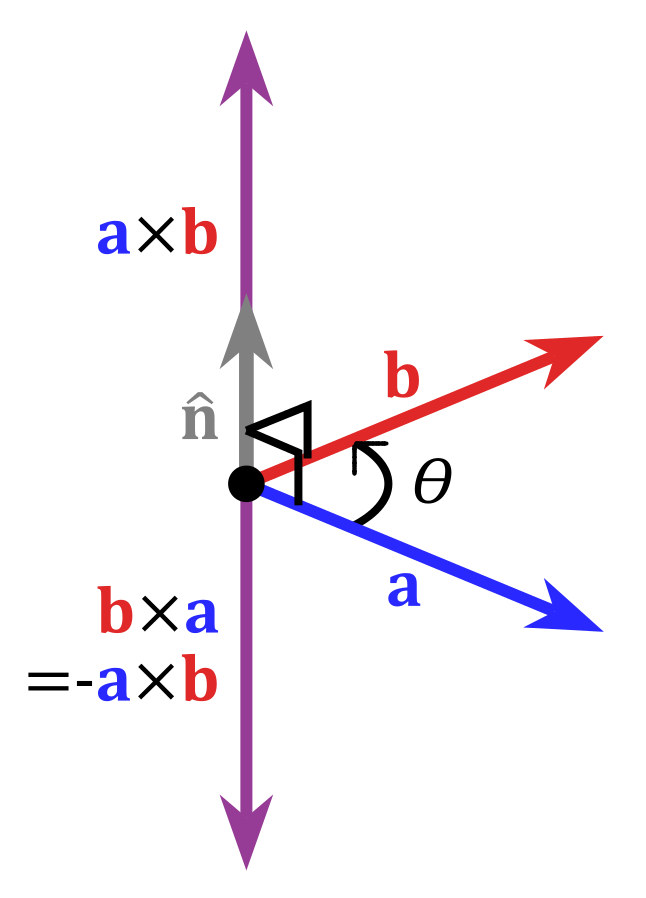
\includegraphics[width=0.3\linewidth]{crossprod.png}}

for $a, b \in \mathbb{R}^2$:
\[ a \times b = || a || \cdot || b || \cdot n (a, b) \cdot \sin\left( \theta(a, b)  \right), \]
where 
\begin{itemize}
    \item $||v||$ : length of vector $v$
    \item $n(a,b)$ : unit vector perpendicular to $a$ and $b$ (\textit{normal vector}) using the right-hand rule 
    \item $\theta(a, b)$: angle turning $a$ into $b$ (counter-clockwise)
\end{itemize}

When $a, b$ are in the $(x, y)$ plane ($a_z = b_z = 0$), $n$ faces upwards if and only if 
$b$ is in left-plane w.r.t (with respect to) $a$.

\medbreak 

More generally, the $z$ component of $a \times b$ tells us how $b$ relates to $a$:
\begin{itemize}
    \item $z > 0$ : $b$ in the left half-plane w.r.t. $a$
    \item $z < 0$ : $b$ in the right half-plane w.r.t. $a$
    \item $z = 0$ : $a, b$ collinear
\end{itemize}

$a \times b$ can be computed by evaluating the following $3 \times 3$ determinant:
\[ 
\begin{vmatrix}
    i & j & k \\
    a_x & a_y & a_z \\
    b_x & b_y & b_z
\end{vmatrix}  
= 
i \cdot 
\begin{vmatrix}
    a_y & a_z \\
    b_y & b_z
\end{vmatrix}
- j \cdot 
\begin{vmatrix}
    a_x & a_z \\
    b_x & b_z
\end{vmatrix}
+ k \cdot 
\begin{vmatrix}
    a_x & a_y \\
    b_x & b_y
\end{vmatrix},
\]
where $i, j, k$ are the unit vectors in $x, y, z$ directions respectively,
and $|m|$ denotes the determinant of matrix $m$. In particular,
\[
(a \times b)_z = 
\begin{vmatrix}
    a_x & a_y \\
    b_x & b_y
\end{vmatrix}
= a_x \cdot b_y - a_y \cdot b_x 
\]


\subsection*{Orientation Test}
\centerline{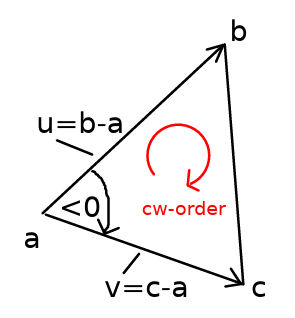
\includegraphics[width=0.3\linewidth]{orientation.png}}

To check whether 3 points are in clockwise order we can use the cross-product:

\medskip 

$a, b, c \in \mathbb{R}^2$ are in clockwise (cw) order if and only if for vectors
$u = b-a$ and $v = c-a$, $v$ lies in the right half-plane w.r.t. $u$,
i.e.,
\[ u_x \cdot v_y - v_x \cdot u_y < 0 \]

Likewise, $a, b, c \in \mathbb{R}^2$ are in counter-clockwise (Ccw) order if and only if
\[ u_x \cdot v_y - v_x \cdot u_y > 0 \]

If $u_x \cdot v_y - v_x \cdot u_y = 0$, the three points are \textit{collinear}, i.e., they lie on a line.

\subsection*{In-Circle Test}
\centerline{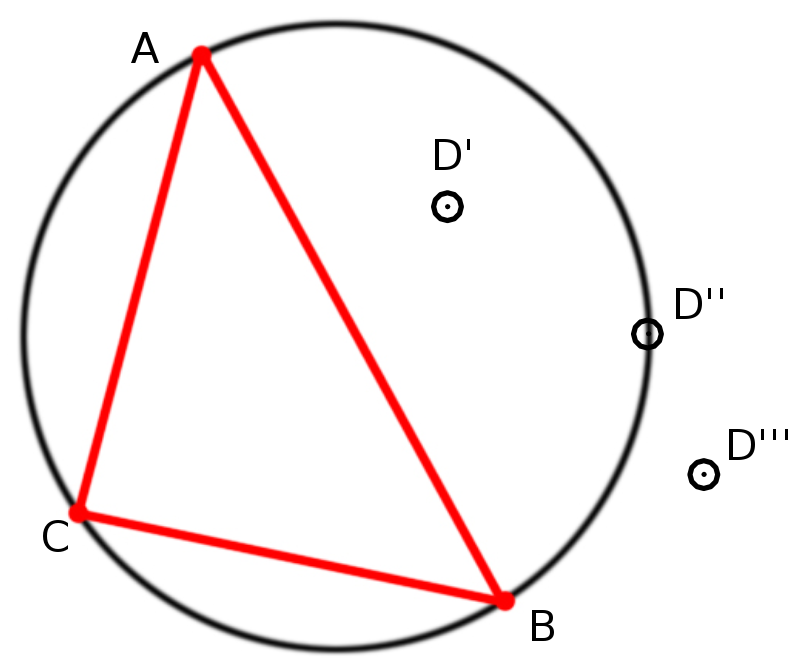
\includegraphics[width=0.3\linewidth]{circle.png}}

It can be shown that $d \in \mathbb{R}^2$ lies inside, on, or outside the circle
defined by $a,b,c \in \mathbb{R}^2$ given in cw order, if the following 4x4
determinant
\[
\begin{vmatrix}
    a_x & a_y & a_x^2 + a_y^2 & 1 \\
    b_x & b_y & b_x^2 + b_y^2 & 1 \\
    c_x & c_y & c_x^2 + c_y^2 & 1 \\
    d_x & d_y & d_x^2 + d_y^2 & 1 
\end{vmatrix}
\]
is $< 0$, $= 0$, $> 0$ respectively. 

\medskip 

If $a, b, c$ are in ccw order, the signes are reversed.

\medskip 

Thus, in-circle tests are basic polynomial computations, which are exact
when using rational arithmetic. No square roots or trigonometric functions are
required!

\medskip

This is useful for detecting beneficial edge flips when generating Delaunay
triangulations.

\linerule


\subsection*{Triangle Mesh Representation}

\begin{itemize}
    \item a triangle mesh is an unordered vector of triangles
    \item triangles are made of points and indexes of neighbouring triangles in the vector
    \item all triangles in a mesh are either oriented cw or ccw
    \item all triangles are contained in a bounding rectangle
    \item outside neighbour index = BORDER (a large constant)
\end{itemize}

\centerline{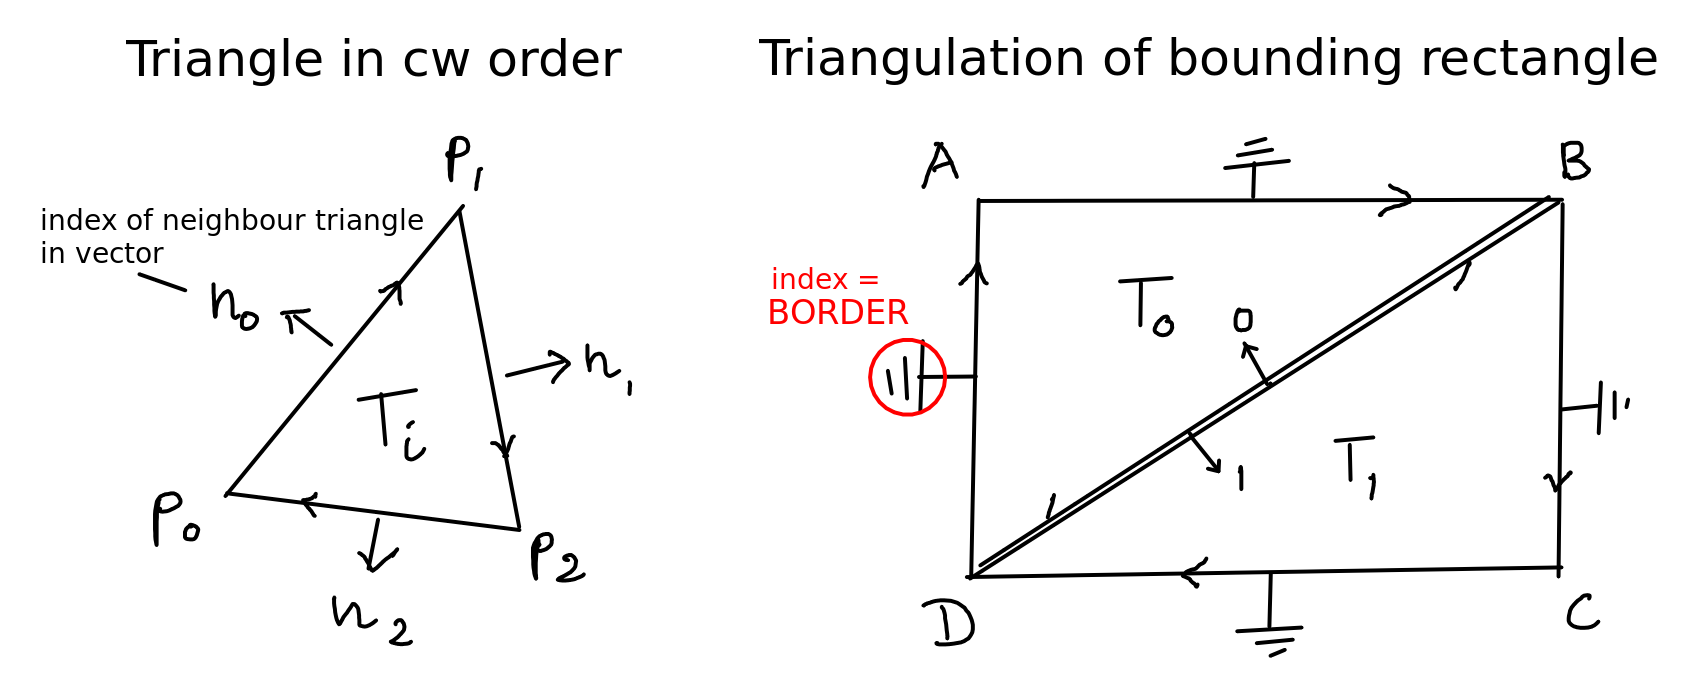
\includegraphics[width=0.9\linewidth]{triang.png}}


\linerule

1. Look at \texttt{Triang.h} and \texttt{Triang.cpp}. 
Implement the tests for functions \texttt{orientation\_test} and \texttt{in\_circle} in \texttt{test.cpp}

\linerule 

2. Implement and test function \texttt{rectangle\_test} in \texttt{test.cpp}


\end{document}